%%%%%%%%%%%%%%%%%%%%%%%%%%%%%%%%%%%%%%%%%%%%%%%%%%%%%%%%%%%%%%%%%%%%%%
\section{AI Agent Improvement}

This project adopted a human-supervised framework to iteratively improve an AI-assisted database engineering agent. Rather than repeatedly modifying generated experiment results, the framework continuously refines the reusable knowledge used by the agent through iterative experiment result generation, evaluation, and knowledge refinement.

The framework clearly separates experiment artifacts from the final project deliverables. During each experiment round, an experiment result is generated solely for evaluation and knowledge refinement. These experiment results are not submitted as project deliverables. Instead, the accumulated knowledge extracted from multiple experiment rounds is incorporated into the Global Agent and section-specific Skills. Based on this refined knowledge, the project team manually prepares, reviews, and finalizes the deliverables stored in the \texttt{output/} directory.

%%%%%%%%%%%%%%%%%%%%%%%%%%%%%%%%%%%%%%%%%%%%%%%%%%%%%%%%%%%%%%%%%%%%%%
\subsection{Experiment Framework}

The experiment framework follows an iterative workflow that continuously improves reusable knowledge throughout the project. Each experiment round generates an experiment result using the current Global Agent together with the corresponding section-specific Skill. The generated experiment result is then evaluated, reusable improvements are identified, and the accumulated knowledge is refined before the next experiment round begins.

%%%%%%%%%%%%%%%%%%%%%%%%%%%%%%%%%%%%%%%%%%%%%%%%%%%%%%%%%%%%%%%%%%%%%%
\subsubsection{Repository Organization}

Figure~\ref{fig:repository-organization} illustrates the repository organization adopted in this project.

\begin{figure}[ht]
    \centering
    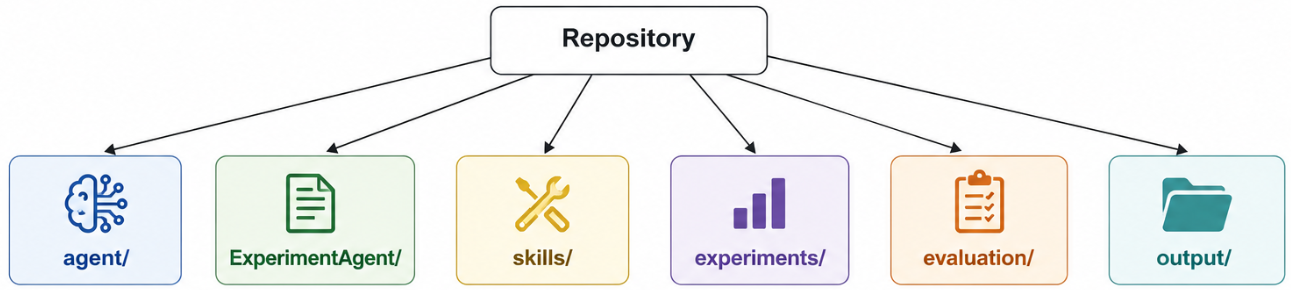
\includegraphics[width=0.95\linewidth]{img/repo-structure.png}
    \caption{Repository organization.}
    \label{fig:repository-organization}
\end{figure}

The repository is organized into four major categories.

\begin{itemize}

    \item \textbf{Project Resources} (\texttt{doc/}, \texttt{report/})

    Contains the project specification, supporting documents, and report source files.

    \item \textbf{Reusable Knowledge} (\texttt{agent/}, \texttt{skills/})

    Stores reusable project-wide knowledge together with section-specific methodologies.

    \item \textbf{Experiment Artifacts} (\texttt{ExperimentAgent/}, \texttt{evaluation/}, \texttt{experiments/})

    Contains the experiment workflow, evaluation rubrics, experiment results, and improvement records produced during iterative refinement.

    \item \textbf{Final Deliverables} (\texttt{output/})

    Stores the final human-produced project deliverables submitted for the course.

\end{itemize}

This organization clearly separates reusable knowledge, experiment artifacts, and final deliverables, allowing the experiment framework to evolve independently without affecting the submitted project outputs.


%%%%%%%%%%%%%%%%%%%%%%%%%%%%%%%%%%%%%%%%%%%%%%%%%%%%%%%%%%%%%%%%%%%%%%
\subsubsection{Experiment Workflow}

For each project section, the experiment proceeds as follows.

\begin{enumerate}

    \item Read the project requirements and supporting documents.

    \item Generate or update the section-specific Skill.

    \item Generate an experiment result using the current Global Agent and the corresponding Skill.

    \item Evaluate the experiment result using predefined evaluation criteria.

    \item Record identified weaknesses together with reusable improvement suggestions.

    \item Update the corresponding Skill and, when appropriate, the Global Agent.

    \item Repeat the process for the next experiment round.

\end{enumerate}

Rather than directly revising experiment results, the framework continuously improves the reusable knowledge used to generate subsequent experiment results.

%%%%%%%%%%%%%%%%%%%%%%%%%%%%%%%%%%%%%%%%%%%%%%%%%%%%%%%%%%%%%%%%%%%%%%
\subsubsection{Experiment Agents}

The experiment workflow is implemented by six specialized agents located in the \texttt{ExperimentAgent/} directory. Each agent performs a dedicated responsibility within the iterative improvement process, allowing knowledge generation, evaluation, and refinement to remain modular and reusable across different project sections.

\begin{table}[H]
\centering
\caption{Responsibilities of experiment agents}
\label{tab:experiment-agents}

\renewcommand{\arraystretch}{1.25}

\begin{tabularx}{\linewidth}{|>{\ttfamily\raggedright\arraybackslash}p{4.4cm}|X|}
\hline

\textbf{Agent}
&
\textbf{Responsibility}
\\
\hline

00-experiment-policy
&
Defines the experiment rules, repository constraints, and human-supervised operating principles.
\\
\hline

01-workflow
&
Determines the current experiment phase and coordinates the overall experiment workflow.
\\
\hline

02-skill-builder
&
Creates or updates section-specific Skills using accumulated improvement knowledge from previous experiment rounds.
\\
\hline

03-result-generator
&
Generates an experiment result using the current Global Agent together with the corresponding Skill.
\\
\hline

04-evaluate
&
Evaluates the experiment result according to predefined evaluation criteria and identifies deficiencies.
\\
\hline

05-improve
&
Summarizes evaluation findings, identifies root causes, and proposes reusable updates for the Global Agent or the corresponding Skill.
\\
\hline

\end{tabularx}

\end{table}

The modular design enables each agent to evolve independently while maintaining a consistent experiment workflow. Throughout the project, experiment results serve only as intermediate artifacts for evaluation and knowledge refinement, whereas the accumulated knowledge stored in the Global Agent and Skills forms the foundation for producing the final human-reviewed project deliverables.

%%%%%%%%%%%%%%%%%%%%%%%%%%%%%%%%%%%%%%%%%%%%%%%%%%%%%%%%%%%%%%%%%%%%%%
\subsection{Agent Architecture}

The proposed framework adopts a modular architecture that separates reusable knowledge from experiment artifacts. Instead of embedding all project knowledge within a single prompt, the framework organizes reusable knowledge into independent components with clearly defined responsibilities. This separation improves maintainability, enables localized refinement, and preserves the evolution history of the Agent throughout the experiment.

%%%%%%%%%%%%%%%%%%%%%%%%%%%%%%%%%%%%%%%%%%%%%%%%%%%%%%%%%%%%%%%%%%%%%%
\subsubsection{Architecture Overview}

Figure~\ref{fig:architecture} illustrates the architecture of the proposed agent improvement framework.

\begin{figure}[ht]
    \centering
    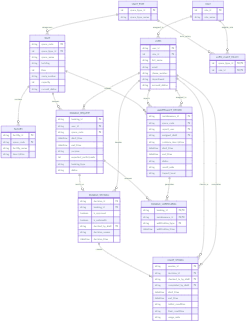
\includegraphics[width=0.75\linewidth]{img/4.2.1.architect_overview.png}
    \caption{Architecture of the proposed agent improvement framework.}
    \label{fig:architecture}
\end{figure}

The proposed framework separates reusable knowledge, experiment results, and knowledge refinement into independent components. The \textit{Global Agent} stores reusable project-wide knowledge shared across all project sections, while each \textit{Section-specific Skill} contains methodologies and verification procedures for a specific project section.

During each experiment round, the project specification, the Global Agent, and the corresponding Skill are combined to generate an experiment result. The generated experiment result is first evaluated according to predefined evaluation criteria and is subsequently reviewed by human evaluators to verify correctness, consistency, and requirement coverage.

The evaluation findings are summarized in an \texttt{ImproveXX} document, which records identified weaknesses, root causes, and reusable improvement proposals. Section-specific improvements are incorporated into the corresponding Skill, whereas project-wide improvements are incorporated into the Global Agent before the next experiment round begins.

This architecture enables reusable knowledge to evolve continuously while preserving experiment results as immutable experiment artifacts. Consequently, improvements accumulated throughout the experiment are inherited by subsequent experiment rounds without modifying previously generated experiment results.

%%%%%%%%%%%%%%%%%%%%%%%%%%%%%%%%%%%%%%%%%%%%%%%%%%%%%%%%%%%%%%%%%%%%%%
\subsubsection{Component Responsibilities}

Table~\ref{tab:components} summarizes the responsibilities of each component.

\begin{table}[H]
\centering
\renewcommand{\arraystretch}{1.35}
\caption{Responsibilities of framework components}
\label{tab:components}

\begin{tabularx}{\linewidth}{|>{\raggedright\arraybackslash}p{3.5cm}|X|}
\hline

\textbf{Component}
&
\textbf{Responsibility}
\\
\hline

Global Agent
&
Stores reusable project-wide knowledge shared across all project sections, including requirement traceability, naming conventions, verification strategies, and anti-hallucination rules.
\\
\hline

Section Skills
&
Store reusable methodologies, workflows, verification checklists, and common mistakes specific to individual project sections.
\\
\hline

Result Generator
&
Produces experiment results using the current version of the Global Agent together with the corresponding Skill.
\\
\hline

Human Evaluation
&
Evaluates experiment results using predefined evaluation rubrics, identifies deficiencies, and determines appropriate improvements.
\\
\hline

Improvement Knowledge
&
Captures reusable lessons learned from evaluation and updates either the Global Agent or the corresponding Skill before the next experiment round.
\\
\hline

\end{tabularx}

\end{table}

%%%%%%%%%%%%%%%%%%%%%%%%%%%%%%%%%%%%%%%%%%%%%%%%%%%%%%%%%%%%%%%%%%%%%%
\subsubsection{Knowledge Refinement}

The framework distinguishes between project-wide knowledge and section-specific knowledge.

Project-wide improvements, such as naming conventions, requirement traceability, or verification strategies, are incorporated into the Global Agent because they benefit every project section. In contrast, improvements related to a specific task, such as ERD construction or SQL implementation, are incorporated only into the corresponding Skill.

This separation minimizes unnecessary coupling between project sections and allows each Skill to evolve independently while maintaining overall consistency through the shared Global Agent.

%%%%%%%%%%%%%%%%%%%%%%%%%%%%%%%%%%%%%%%%%%%%%%%%%%%%%%%%%%%%%%%%%%%%%%
\subsubsection{Knowledge Flow}

Figure~\ref{fig:architecture} also illustrates how knowledge flows through the framework.

At the beginning of each experiment round, the Global Agent and the corresponding Skill are combined to generate an experiment result. The experiment result is then evaluated by human reviewers, who identify weaknesses and summarize reusable improvements. These improvements are incorporated into the knowledge base before the following experiment round begins.

Consequently, experiment results remain immutable experiment artifacts, while the Global Agent and Skills continuously evolve throughout the project. This design allows improvements to accumulate across multiple experiment rounds without modifying previously generated experiment results.

%%%%%%%%%%%%%%%%%%%%%%%%%%%%%%%%%%%%%%%%%%%%%%%%%%%%%%%%%%%%%%%%%%%%%%
\subsection{Iterative Improvement}

The objective of the experiment is to continuously improve the reusable knowledge of the AI agent rather than directly modifying generated experiment results. Each experiment cycle evaluates the current capability of the Global Agent and section-specific Skills, identifies reusable improvements, and incorporates these improvements into the knowledge base before the next experiment result is generated.

Throughout the project, experiment results serve only as intermediate artifacts for evaluation and knowledge refinement, while the accumulated knowledge stored in the Global Agent and Skills is progressively refined across multiple experiment rounds.

%%%%%%%%%%%%%%%%%%%%%%%%%%%%%%%%%%%%%%%%%%%%%%%%%%%%%%%%%%%%%%%%%%%%%%
\subsubsection{Improvement Cycle}

Figure~\ref{fig:iteration} illustrates the iterative improvement process adopted in this project.

\begin{figure}[ht]
    \centering
    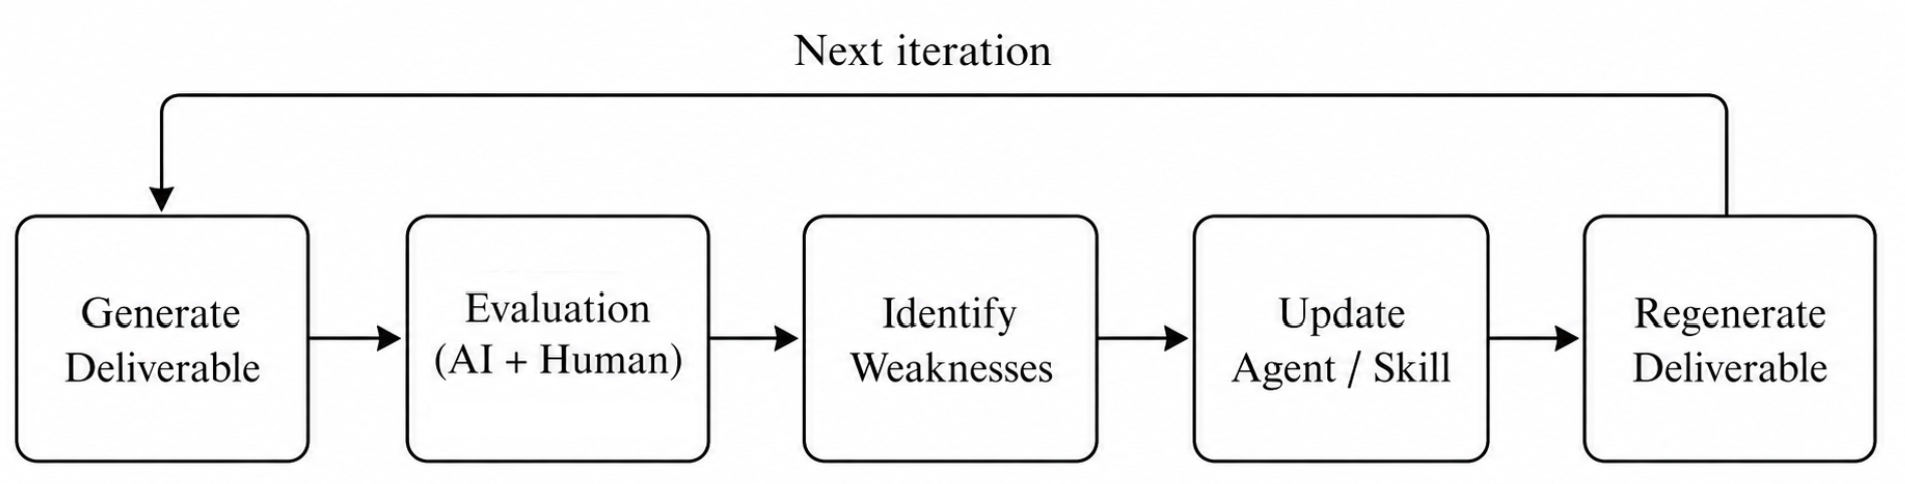
\includegraphics[width=\linewidth]{img/4.3.1.png}
    \caption{Iterative improvement process.}
    \label{fig:iteration}
\end{figure}

Each improvement cycle consists of the following activities.

\begin{enumerate}

    \item Read the project requirements together with the current version of the Global Agent and the corresponding Skill.

    \item Generate an experiment result for the target project section.

    \item Evaluate the experiment result using the predefined evaluation criteria.

    \item Summarize the evaluation findings in an \texttt{ImproveXX} document, including identified weaknesses, root causes, and reusable improvement proposals.

    \item Update the corresponding Skill using the recorded improvements.

    \item Update the Global Agent only when an improvement is applicable across multiple project sections.

    \item Generate the next experiment result using the updated knowledge.

\end{enumerate}

Unlike conventional document revision, experiment results are not manually rewritten. Instead, evaluation feedback is transformed into reusable knowledge that improves subsequent experiment rounds.

%%%%%%%%%%%%%%%%%%%%%%%%%%%%%%%%%%%%%%%%%%%%%%%%%%%%%%%%%%%%%%%%%%%%%%
\subsubsection{Knowledge Evolution}

The experiment distinguishes between two categories of reusable improvements.

\begin{itemize}

\item \textbf{Section-specific improvements}

These improvements are incorporated into the corresponding Skill. Examples include methodologies for business requirement analysis, ERD construction, logical schema mapping, SQL implementation, and query design.

\item \textbf{Project-wide improvements}

These improvements are incorporated into the Global Agent because they are applicable across multiple project sections. Typical examples include naming conventions, requirement traceability, consistency verification, and anti-hallucination guidelines.

\end{itemize}

This separation enables each Skill to evolve independently while maintaining overall consistency through the shared Global Agent.

%%%%%%%%%%%%%%%%%%%%%%%%%%%%%%%%%%%%%%%%%%%%%%%%%%%%%%%%%%%%%%%%%%%%%%
\subsubsection{Representative Improvement History}

Table~\ref{tab:history} summarizes representative improvements identified during the experiment.

\begin{table}[H]
\centering

\renewcommand{\arraystretch}{1.35}
\caption{Representative improvement history}
\label{tab:history}

\begin{tabularx}{\linewidth}
{
>{\raggedright\arraybackslash}p{3.5cm}
X
}

\toprule

\textbf{Improvement Category}
&
\textbf{Representative Improvements}

\\

\midrule

Requirement Analysis
&
Improved extraction of actors, business rules, operational constraints, and exceptional cases before database design.
\\

Consistency
&
Introduced unified naming conventions and terminology shared across all project sections.
\\

Requirement Traceability
&
Added explicit verification to ensure that important design decisions could be traced back to the project specification.
\\

Design Validation
&
Strengthened validation procedures to verify consistency between the ERD, relational schema, SQL implementation, and query design.
\\

Verification
&
Expanded section-specific verification checklists to reduce omissions and unsupported assumptions during experiment result generation.
\\

\bottomrule

\end{tabularx}

\end{table}

%%%%%%%%%%%%%%%%%%%%%%%%%%%%%%%%%%%%%%%%%%%%%%%%%%%%%%%%%%%%%%%%%%%%%%
\subsubsection{Experiment Results}

Table~\ref{tab:progress} summarizes the evaluation scores of experiment results obtained during the three experiment rounds.

\begin{table}[H]

\centering

\caption{Evaluation scores of experiment results}

\label{tab:progress}

\begin{tabularx}{\linewidth}{lccc}

\toprule

\textbf{Project Section}
&
\textbf{Round 1}
&
\textbf{Round 2}
&
\textbf{Round 3}

\\

\midrule

01 Business Requirement Analysis
&
7.2
&
8.2
&
9.5
\\

02 Conceptual Database Design
&
8.5
&
9.0
&
9.5
\\

03 Logical Database Design
&
8.0
&
9.0
&
9.8
\\

04 Database Design Validation
&
7.5
&
8.5
&
9.0
\\

05 Database Implementation
&
7.5
&
8.8
&
9.3
\\

06 Sample Data Preparation
&
7.5
&
8.8
&
9.0
\\

07 Query Design
&
7.2
&
8.5
&
10.0
\\

\bottomrule

\end{tabularx}

\end{table}

The evaluation results demonstrate consistent improvement across all project sections. As reusable knowledge accumulated through successive experiment rounds, experiment results became progressively more complete, consistent, and required fewer revisions during evaluation. These improvements indicate that the experiment successfully enhanced the reusable knowledge stored in the Global Agent and section-specific Skills rather than optimizing individual experiment results.

%%%%%%%%%%%%%%%%%%%%%%%%%%%%%%%%%%%%%%%%%%%%%%%%%%%%%%%%%%%%%%%%%%%%%%
\subsection{Evaluation}

Each experiment result generated during the experiment was evaluated before the next iteration began. A fixed evaluation methodology was adopted to ensure that experiment results could be assessed consistently across different project sections and experiment rounds. Rather than directly correcting experiment results, the evaluation process focused on identifying reusable improvements that could be incorporated into the Global Agent or the corresponding Skill.

%%%%%%%%%%%%%%%%%%%%%%%%%%%%%%%%%%%%%%%%%%%%%%%%%%%%%%%%%%%%%%%%%%%%%%
\subsubsection{Evaluation Criteria}

Table~\ref{tab:criteria} summarizes the evaluation criteria adopted throughout the experiment.

\begin{table}[H]
\centering
\renewcommand{\arraystretch}{1.35}
\caption{Evaluation criteria}
\label{tab:criteria}

\begin{tabularx}{\linewidth}{>{\raggedright\arraybackslash}p{4cm}X}

\toprule

\textbf{Criterion}
&
\textbf{Description}

\\

\midrule

Requirement Coverage
&
Evaluates whether functional requirements and business rules from the project specification are correctly represented in the generated experiment result.
\\

Correctness
&
Assesses the correctness of entities, relationships, constraints, SQL statements, and other database design decisions.
\\

Consistency
&
Verifies consistent terminology, naming conventions, and logical consistency across all project artifacts.
\\

Requirement Traceability
&
Checks whether major design decisions can be traced back to explicit project requirements.
\\

Completeness
&
Evaluates whether the generated experiment result contains all expected components for the corresponding project section.
\\

Hallucination Prevention
&
Ensures that generated information is supported by the project specification rather than unsupported assumptions.
\\

\bottomrule

\end{tabularx}

\end{table}

The same evaluation criteria were applied throughout the entire experiment, ensuring that experiment results could be evaluated consistently across successive experiment rounds.

%%%%%%%%%%%%%%%%%%%%%%%%%%%%%%%%%%%%%%%%%%%%%%%%%%%%%%%%%%%%%%%%%%%%%%
\subsubsection{Evaluation Procedure}

Each experiment result was evaluated using the following procedure.

\begin{enumerate}

\item Compare the generated experiment result against the project specification.

\item Evaluate the experiment result using the predefined evaluation criteria.

\item Identify missing requirements, inconsistencies, unsupported assumptions, and implementation errors.

\item Record the findings in the corresponding evaluation report.

\item Summarize reusable improvements in the associated \texttt{ImproveXX} document.

\item Update the corresponding Skill and, when applicable, the Global Agent before the next experiment round.

\end{enumerate}

By keeping the evaluation procedure unchanged throughout the experiment, improvements observed across successive experiment rounds primarily reflect refinements to reusable knowledge rather than changes in the evaluation methodology.

%%%%%%%%%%%%%%%%%%%%%%%%%%%%%%%%%%%%%%%%%%%%%%%%%%%%%%%%%%%%%%%%%%%%%%
\subsubsection{Evaluation Results}

The evaluation results presented in Table~\ref{tab:progress} demonstrate that the quality of experiment results improved consistently across successive experiment rounds. The largest improvements were observed in project sections requiring extensive requirement analysis and verification, including Business Requirement Analysis, Database Implementation, and Query Design.

The progressive improvement in experiment result quality indicates that the accumulated knowledge stored in the Global Agent and section-specific Skills effectively reduced omissions, inconsistencies, and unsupported assumptions during subsequent experiment rounds. Rather than repeatedly correcting experiment results, the framework continuously improved the reusable knowledge used to generate them.

%%%%%%%%%%%%%%%%%%%%%%%%%%%%%%%%%%%%%%%%%%%%%%%%%%%%%%%%%%%%%%%%%%%%%%
\subsubsection{Threats to Validity}

Several limitations should be considered when interpreting the experimental results.

\begin{itemize}

\item The experiment was conducted using a single database engineering case study. Additional case studies would be required to evaluate the generalizability of the proposed framework.

\item Evaluation of experiment results relied on human reviewers. Although predefined rubrics were applied consistently, some assessment decisions inevitably involved subjective judgment.

\item The experiment focused on iterative knowledge refinement and did not compare different prompting strategies, language models, or autonomous agent architectures under identical experimental conditions.

\item The reported evaluation scores provide relative evidence of improvement within this project rather than absolute measures of AI capability.

\end{itemize}

Despite these limitations, the experiment demonstrates that systematic human-supervised refinement can effectively improve the reusable knowledge of an AI-assisted database engineering agent. By incorporating evaluation feedback into the Global Agent and section-specific Skills, the framework progressively improved the quality of experiment results while preserving reproducible experiment artifacts. The final deliverables submitted for the course were manually reviewed and prepared by the project team based on the accumulated knowledge obtained throughout the experiment.
